\documentclass{beamer}
\usetheme{}
\usecolortheme{dolphin}           
\useinnertheme{circles}
\setbeamertemplate{itemize items}[default]
\setbeamertemplate{enumerate items}[default]
\usepackage[T1]{fontenc}
\usepackage[utf8]{inputenc}
\usepackage{lmodern}
\usepackage{amsmath}
\usepackage{booktabs} 
\usepackage{graphicx}        
\usepackage{array}
\usepackage{color}
\usepackage{textcomp}
\usepackage{epstopdf}                     % For EPS figures
\makeatletter
\def\zapcolorreset{\let\reset@color\relax\ignorespaces}
\def\colorrows#1{\noalign{\aftergroup\zapcolorreset#1}\ignorespaces}
\makeatother
\graphicspath{{/home/swl/Dropbox/ucd/international_trade/tex/}} 
\setbeamertemplate{navigation symbols}{}

%--------------------------------------
%%%% DETAILS TITLE PAGE %%%%
%--------------------------------------
\title{Political economy of international trade}
\author{School of Economics, University College Dublin}
\date{Autumn 2017}
\begin{document}
%--------------------------------------
%%%% TITLE SLIDE %%%%
%--------------------------------------
\begin{frame}
\titlepage  
\end{frame}

%--------------------------------------
\begin{frame}
  Economists are nearly unanimous in opposition against protectionism
  \begin{itemize}
    \item Save some heterodox economists
  \end{itemize}
  \medskip
  Yet protectionist measures persist 
  \begin{itemize}
    \item EU's Common Agricultural Policy
    \item Steel tariffs in the US
  \end{itemize}  
  \medskip
  Protectionism is mainly used for producers.   
\end{frame}
%--------------------------------------

\begin{frame}
Governments generally prefer tariffs and import quotas over production subsidies which is peculiar since
  \begin{enumerate}
    \item Lump-sum tax transfers are more efficient
    \item Avoids consumption costs of production
  \end{enumerate}
  \medskip
  What explains the discrepancy between research results and implemented policy?
\end{frame}
%--------------------------------------

%--------------------------------------
\begin{frame}
  Two things to keep in mind when analysing trade policies  
  \begin{enumerate}
    \item Economic self interests
    \begin{itemize}
      \item Individuals favour or oppose trade policies based on the effects on real income
    \end{itemize}
    \item Social concerns
    \begin{itemize}
      \item The government's concern for welfare and the desire to promote national and international goals
    \end{itemize}
  \end{enumerate}
\end{frame}
%--------------------------------------

%--------------------------------------
\begin{frame}
  Let's consider a standard Heckscher-Ohlin where the imported good is labour intensive.\\
  \bigskip
  Will there be free trade or protectionism?  
\end{frame}
%--------------------------------------

%--------------------------------------
\begin{frame}
\begin{itemize}
  \item Workers will favour tariff
  \item Capitalist will favour free trade
\end{itemize}
\medskip  
  Under majority voting rule protectionism will be the more likely outcome
  \begin{align*}
    Number\;of\;Workers > Number\;of\;Capitalists
  \end{align*}    
\end{frame}
%--------------------------------------

%--------------------------------------
\begin{frame}
Under some circumstances free trade can be the preferred option
  \begin{itemize}
    \item The gains from trade can be redistributed to compensate the losers, while still being better off than under protectionism
  \end{itemize}  
  \medskip
  So protectionism will be chosen when
  \begin{align*}
    Redistribution\;costs + Compensation\;costs > Capitalists\;gains 
  \end{align*}
\end{frame}
%--------------------------------------

%--------------------------------------
\begin{frame}
  Voting costs can also lead to protectionism
  \begin{itemize}
    \item Think of situation where the benefits from free trade are relatively small for many individuals
  \end{itemize}  
\end{frame}
%--------------------------------------

%--------------------------------------
\begin{frame}
Let's consider a Specific Factors model where capital and labour are the industry-specific factors and where
  \begin{itemize}
    \item The sector subject to competition under free trade incurs losses larger than voting costs
    \item The sector that benefits from free trade has gains and protection costs smaller than voting costs
  \end{itemize}
  \medskip
\begin{enumerate}
  \item A comparatively small number of people in the hurt industry will vote in favour or protection
  \item Large number of people in other sector might not be bothered to vote 
\end{enumerate}  
\end{frame}
%--------------------------------------

%--------------------------------------
\begin{frame}
  We can explain the existence of protectionism using two approaches
  \begin{enumerate}
    \item Median voter theorem
    \item Collective action
  \end{enumerate}
\end{frame}
%--------------------------------------

%--------------------------------------
\begin{frame}
  Let's assume that we have a two-party system with Conservatives $C$ and Labour $L$ and a continuum of voters with size $N$.
  \begin{itemize}
    \item Voters are lined up by their preferred tariff rate: uniform distribution between $0-T$
  \end{itemize}
  \medskip
  \begin{enumerate}
    \item Choose party closest to preferred tariff rate
    \item Party takes tariff position to maximise support
  \end{enumerate}
\end{frame}
%--------------------------------------

%--------------------------------------
\begin{frame}{Median voter theorem}
  \begin{figure}
    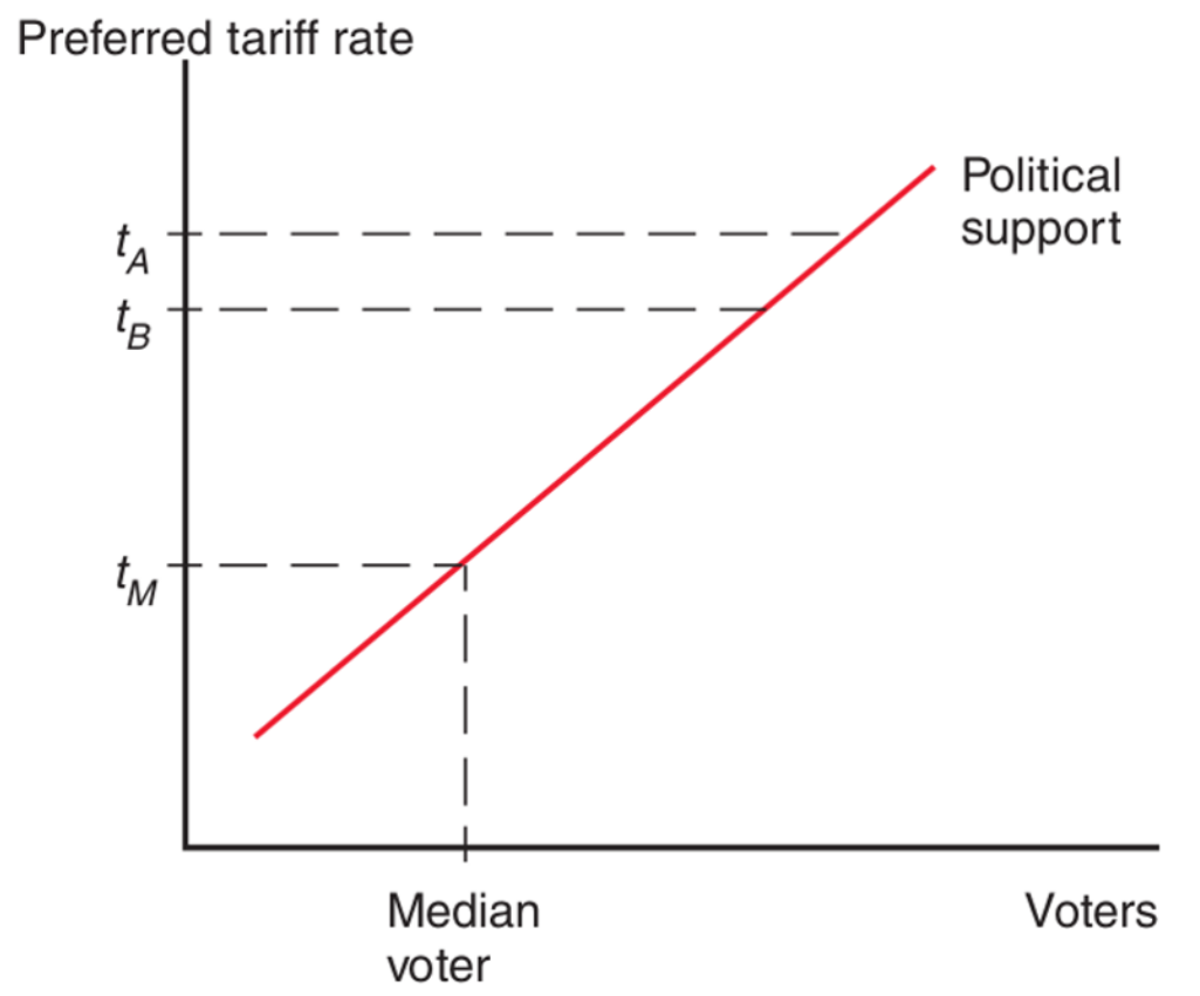
\includegraphics{median_voter}
  \end{figure}
\end{frame}
%--------------------------------------

%--------------------------------------
\begin{frame}
  Median voter theorem predicts that both parties will pick the same median voter supported trade policy. \\
  This contrasts with observed trade policies
  \begin{itemize}
    \item Typically trade policies help industry a lot, but hurts everyone a little
  \end{itemize}
  \medskip
  Collective action might offer a better explanation considering that trade policy is a public good.    
\end{frame}
%--------------------------------------

%--------------------------------------
\begin{frame}
  Let's consider the EU's Common Agricultural Policy which means that every EU consumer pays too much for most of their food. 
  From the perspective of the average consumer
  \begin{itemize}
    \item Benefit from having subsidy removed is relatively small
    \item Probability of collective action having an effect is relatively small
  \end{itemize}
  \medskip
  Although the cost of taking action is also small, the average consumer won't take actions  
\end{frame}
%--------------------------------------

%--------------------------------------
\begin{frame}
Things look different from the perspective of the average farmer
\begin{itemize}
    \item Benefit from keeping subsidy is relatively large
    \item Probability of action having effect is relatively large
  \end{itemize}
  \medskip
  Given that the cost of taking action is relatively small, the farmer will take action
\end{frame}
%--------------------------------------

%--------------------------------------
\begin{frame}{Farmers' collective action}
  \begin{figure}
    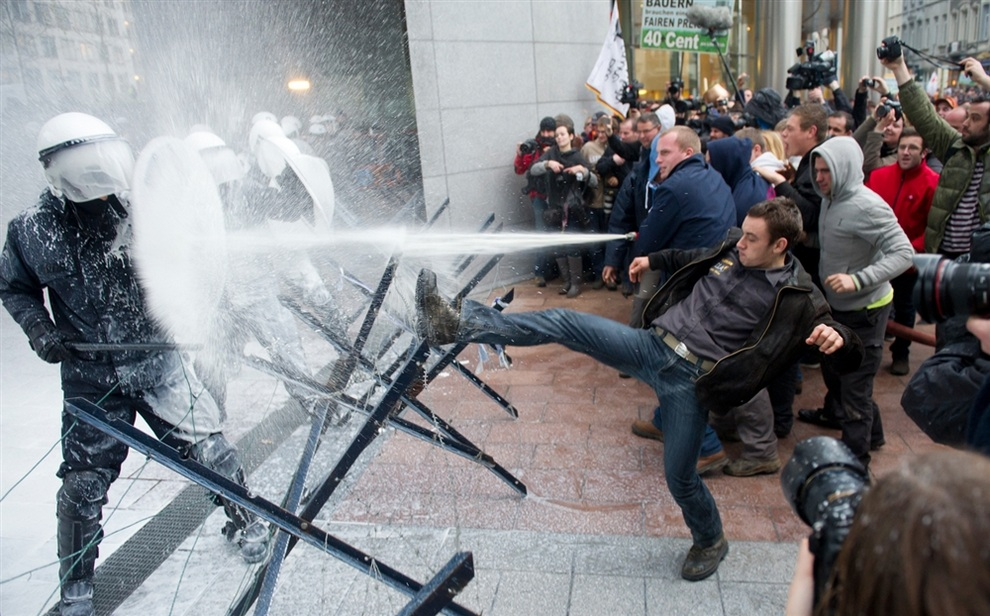
\includegraphics[scale=.4]{collective_action}
  \end{figure}
\end{frame}
%--------------------------------------

%--------------------------------------
\begin{frame}
  Policies with a large aggregate loss but small individual losses are difficult to change.
  Whereas small groups with concentrated losses are more willing to pay the effort-fixed cost.
  This leads to a free rider problem with public goods
  \begin{itemize}
    \item Consumer believes its contribution is too small to affect policy outcome
    \item Dominant strategy is not to bother
    \item Everyone ends up worse
  \end{itemize}
\end{frame}
%--------------------------------------

%--------------------------------------
\begin{frame}
  Policies also persist due to the incentives faced by the politicians who win elections by
  \begin{enumerate}
    \item Advocating popular policies (median voter theorem)
    \item Have funds to run campaigns (collective action)
  \end{enumerate}
  \medskip
  As a result trade policy is influenced by well-organised groups with concentrated gains who are more likley to overcome the free rider problem 
\end{frame}
%--------------------------------------

%--------------------------------------
\begin{frame}
  Let's have a look a country's economic self interest. 
  Consider two countries: San Marcos and Nambutu
  \begin{itemize}
    \item Each country can protect its producers by setting a tariff
    \item A country's reaction depends on the other country's policy
  \end{itemize}  
\end{frame}
%--------------------------------------

%--------------------------------------
\begin{frame}
  \begin{table}
    \begin{tabular}{lcc}
    ~ &\multicolumn{2}{c}{\textbf{San Marcos}}\\
    \textbf{Nambutu}  & Free trade & Tariff\\
    Free trade  & 100, 100  & -100, 200\\
    Tariff  & ~ & ~\\      
    \end{tabular}
  \end{table}
\end{frame}
%--------------------------------------

%--------------------------------------
\begin{frame}
  \begin{table}
    \begin{tabular}{lcc}
    ~ &\multicolumn{2}{c}{\textbf{San Marcos}}\\
    \textbf{Nambutu}  & Free trade & Tariff\\
    Free trade  & ~ & ~\\
    Tariff  & 200, -100 & -50,-50 ~\\      
    \end{tabular}
  \end{table}
\end{frame}
%--------------------------------------

%--------------------------------------
\begin{frame}
  \begin{table}
    \begin{tabular}{lcc}
    ~ &\multicolumn{2}{c}{\textbf{San Marcos}}\\
    \textbf{Nambutu}  & Free trade & Tariff\\
    Free trade  & 100, 100  & -100, 200\\
    Tariff  & 200,-100 & -50, -50\\      
    \end{tabular}
  \end{table}
\end{frame}
%--------------------------------------

%--------------------------------------
\begin{frame}
  In setting the tariffs the countries can have a cooperative equilibrium, but there is also a non-cooperative equilibrium leading to the risk of prisoner's dilemma
  \begin{itemize}
    \item Tariff will be the dominant strategy
    \item Results in global welfare costs
  \end{itemize}
  \medskip
  This illustrates the need for trade negotiations
  \begin{itemize}
    \item Can help avoid trade wars as countries enact trade restrictions
  \end{itemize}
\end{frame}
%--------------------------------------

%--------------------------------------
\begin{frame}
  Using trade negotiations there are two ways to liberalise trade
  \begin{enumerate}
    \item Bilateral or regional agreements
    \item Multilateral agreements
  \end{enumerate}  
\end{frame}
%--------------------------------------

%--------------------------------------
\begin{frame}
  Consider three countries $-$ Germany, Brazil, and Japan $-$ with the following bargaining goals
  \medskip
  \begin{enumerate}
    \item Germany wants to reduce Brazil's pharmaceutical tariff
    \item Brazil want to reduce Japan's wheat tariff
    \item Japan wants to reduce Germany's car tariff
  \end{enumerate}
\end{frame}
%--------------------------------------

%--------------------------------------
\begin{frame}
  The first option is to hold bilateral negotiations
  \begin{enumerate}
    \item Germany-Brazil: GER wants to reduce BRA pharmaceutical tariff but has nothing to offer
    \item Brazil-Japan: BRA wants to reduce JPN wheat tariff but has nothing to offer
    \item Japan-Germany: JPN wants to reduce GER car tariff but has nothing to offer
  \end{enumerate}
  \medskip
  Likely outcome is that nothing will happen.  
\end{frame}
%--------------------------------------

%--------------------------------------
\begin{frame}
  A second option is to hold multilateral negotiations in which
  \begin{enumerate}
    \item BRA will reduce the tariff on GER's pharmaceutical products
    \item In return GER will convince JPN to reduce the wheat tariff on wheat from BRA, promising that GER will reduce the car tariff for JPN
  \end{enumerate}
  \medskip
  Likely outcome is that each country achieves its goals. 
\end{frame}
%--------------------------------------

%--------------------------------------
\begin{frame}
    Bargaining between multiple countries can lead to better deals.
    Another example 
    \begin{enumerate}
      \item Spain, which produces olive oil
      \item Italy, which produces olive oil
      \item Germany, which consumes olive oil
    \end{enumerate}
    \medskip
    Let's assume that bilateral negotiations between Italy and Germany led to a reduction in the tariff on Italy's olive oil
    \begin{itemize}
      \item Following some quid pro quo principle
    \end{itemize}
\end{frame}
%--------------------------------------

%--------------------------------------
\begin{frame}
  If Germany has market power, the reducing the tariff on Italian olive oil will increase world prices
  \begin{itemize}
    \item Due to an increase in German demand
  \end{itemize}
  \medskip
  This price increase will benefit Italy but also Spain, the other olive oil producer: This is a positive externality
  \begin{itemize}
    \item The effect of tariff reduction is large than accounted for during the trade talks
    \item Meaning that Germany will actually get less in return, and therefore won't reduce the tariff by much
  \end{itemize}
  \medskip
  A solution to this is to internalise the externality, by including Spain in the trade talks. 
\end{frame}
%--------------------------------------

%--------------------------------------
\begin{frame}
  \textbf{EU-Japan trade deal}: agreed in July 2017, bringing together economies accounting for 19\% of global GDP
  \begin{itemize}
    \item Negotiations took 4 years, taking 18 rounds
    \item Includes tariff cuts, cooperation on standard and regulations, and opening up of public procurement markets
  \end{itemize}
  \medskip
  Has also been called the "cars for cheese" deal
  \begin{itemize}
    \item EU sought to reduce Japanese tariffs on meat, wine, and diary products
    \item Japan wanted end to EU import duties on cars
  \end{itemize}
  \medskip
  In the end, the deal was decided by a reduction in EU market demand for soft cheese.
\end{frame}
%--------------------------------------

%--------------------------------------
\begin{frame}
\textbf{Comprehensive Economic and Trade Agreement}, between Canada and EU, signed October 2016, eliminates up to 99\% of tariffs
\begin{itemize}
  \item Took 7 years to complete
  \item Almost failed at last minute due to objections of regional parliament of Wallonia
\end{itemize}
\medskip
Agreement removes customs duties on bilateral exports
\begin{itemize}
  \item For industrial goods and most agricultural products
  \item EU companies can bid for public contracts in Canada
  \item Agreement does not remove non-tariff barriers
\end{itemize}
\medskip
Canada does not have to pay into EU budget, sign up to four freedoms, or abide by European court of justice rulings.
\end{frame}
%--------------------------------------

%--------------------------------------
\begin{frame}
 Some historial background on trade negotiations and the creation of the World Trade Organisation.\\ 
 The 1930s saw tariffs raised to high levels in reaction to the Great Depression.  
 \begin{itemize}
   \item Famously the US Smoot-Hawley tariff act which raised tariffs on 890 items
 \end{itemize}
 \medskip 
 Retaliation by other countries also raising tariffs
\end{frame}
%--------------------------------------

%--------------------------------------
\begin{frame}
Following the Second World War the Bretton Woods institutions were created
\begin{itemize}
  \item IMF, World Bank
  \item General Agreement on Tariffs and Trade (GATT)
\end{itemize}
\medskip
GATT governs trade policy
\end{frame}
%--------------------------------------

%--------------------------------------
\begin{frame}
  Main purpose of GATT
  \begin{enumerate}
    \item Set rules for trade policy
    \item Provide platform for negotiations, on policies and rules
  \end{enumerate}
  \medskip
  Major negotiations take place during Negotiating Rounds
\end{frame}
%--------------------------------------

%--------------------------------------
\begin{frame}
  \textbf{Round 1-5 (1947-61):} Reduced tariffs\\
  \textbf{Round 6 (1964-67):} Kennedy round, reduced tariffs and anti-dumping rules\\  
  \textbf{Round 7 (1973-79):} Tokyo round on tariffs and NTBs\\
  \medskip
  \textbf{Round 8 (1986-94):} Uruguay round which created the WTO
  \begin{itemize}
    \item Besides the usual this round also discussed intellectual property, tariffs concerning textiles and agricultural goods, and it discussed dispute settlement
  \end{itemize}
  \medskip
  Currently we are in round 9 (2001-) or the Doha round, which failed. 
\end{frame}
%--------------------------------------

%--------------------------------------
\begin{frame}
 How do these negotiations take place?
 Let's focus on tariffs: In early rounds tariff cuts were negotiated between principal supplier and principal demander countries
 \begin{itemize}
   \item Cuts were extended to all member states but large countries tended to dominate this process
 \end{itemize} 
\end{frame}
%--------------------------------------

%--------------------------------------
\begin{frame}
Number of ways to reduce tariffs
 \begin{enumerate}
   \item Single rate
   \item Flat-rate percentage reduction, e.g. cutting all tariffs by 25\% over 5 years
   \item Uruguay round approach
   \begin{itemize}
     \item Cut tariffs on agricultural products by 36\%  over 6 years, min. of 15\% on each product of the period
   \end{itemize}
  \item Harmonising reductions  
 \end{enumerate}  
\end{frame}
%--------------------------------------

%--------------------------------------
\begin{frame}
Harmonising reductions are aimed at making steeper cuts for higher tariffs, for instance different percentages for different tariff bands
\begin{itemize}
  \item No cuts on tariffs between 0-10\%, 25\% cuts for tariffs between 11-50\%, etc.  
\end{itemize}
\medskip
Or can use the Swiss formula
 \begin{align*}
   Z=\frac{AX}{(A+X)}
 \end{align*}
 $X$ is original tariff\\
 $A$ coefficient and maximum tariff rate\\
 $Z$ resulting lower tariff rate, at end of period\\
 \begin{itemize}
   \item Proposed by the Swiss during the Tokyo round
   \item Swiss now prefer Uruguay round method
 \end{itemize}
\end{frame}
%--------------------------------------

%--------------------------------------
\begin{frame}
  \begin{figure}
    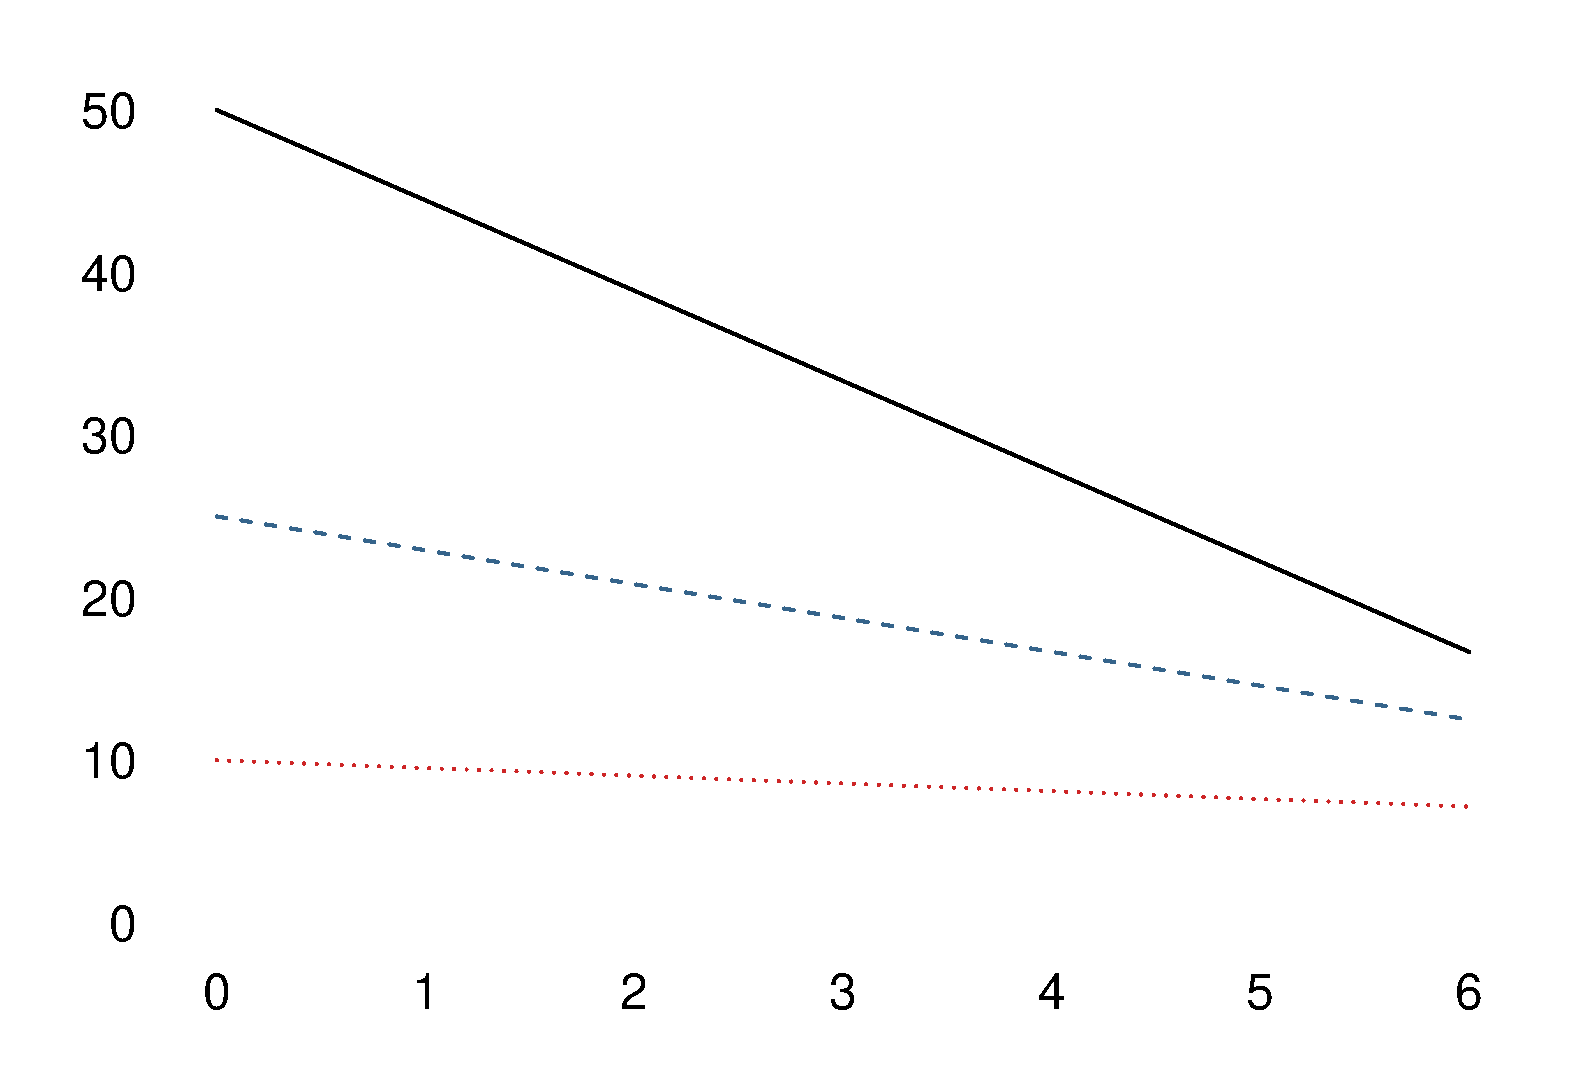
\includegraphics[scale=.4]{swiss_formula.eps}
  \end{figure}
  Swiss formula reduces high tariffs more than low tariffs. 
\end{frame}
%--------------------------------------

%--------------------------------------
\begin{frame}
  Concerning trade rules, negotiations take place in country groupings who draft proposals and then try to persuade others
  \begin{itemize}
    \item Again a process that is dominated by the larger countries.
  \end{itemize}
  \medskip
  Is the WTO bad for smaller countries?
  \begin{enumerate}
    \item They do benefit from rule-of-law
    \item Can increase bargaining power by collaborating
  \end{enumerate}
\end{frame}
%--------------------------------------

%--------------------------------------
\begin{frame}
 WTO consists of three parts
 \begin{enumerate}
   \item GATT (core business)
   \item GATS: General Agreement on Trade in Services
   \item TRIPs agreement: Trade Related aspects of Intellectual Property Rights
 \end{enumerate}
\end{frame}
%--------------------------------------

%--------------------------------------
\begin{frame}
The WTO was established by the 1995 Uruguay round 
  \begin{itemize}
    \item Which removed quotas on textiles and clothing. 
  \end{itemize}
  \medskip
  The last negotiation round $-$ Doha $-$ failed
  \begin{itemize}
    \item US blaming Brazil and India for protectionism
    \item US and EU unwilling to reduce agricultural subsidies
  \end{itemize}
\end{frame}
%--------------------------------------

%--------------------------------------
\begin{frame}
 The aim of the WTO is to gradually eliminate trade barriers addressing existing trade restrictions via three channels
  \begin{enumerate}
    \item Reduction of tariff rates
    \item Binding tariff rates, i.e. no future increases
    \item Elimination and prevention of non-tariff barriers
  \end{enumerate}  
\end{frame}
%--------------------------------------

%--------------------------------------
\begin{frame}
 WTO has two basic principles
 \begin{enumerate}
   \item Most Favoured Nation (MFN)
   \begin{itemize}
     \item Member state should treat each other member states as it treats its MFN
   \end{itemize}
   \item National Treatment
   \begin{itemize}
     \item No discrimination between imports/importers and domestic products/producers
   \end{itemize}
 \end{enumerate}
 \medskip
 Both principles have permitted exceptions
\end{frame}
%--------------------------------------

%--------------------------------------
\begin{frame}  
 The basis of negotiations, which covers everything from tariffs to technical norms, is a reciprocity objective
 \begin{itemize}
   \item Allows balanced deals and emergence of free-trade coalitions
 \end{itemize}
 \medskip
 Despite the efforts made by the WTO there of course still exist preferential agreements as well as non-tariff barriers.
 The WTO therefore also has a role in dispute settlement. 
\end{frame}
%--------------------------------------

%--------------------------------------
\begin{frame}{Sardina Pilchardus Gervais}
  \begin{figure}
    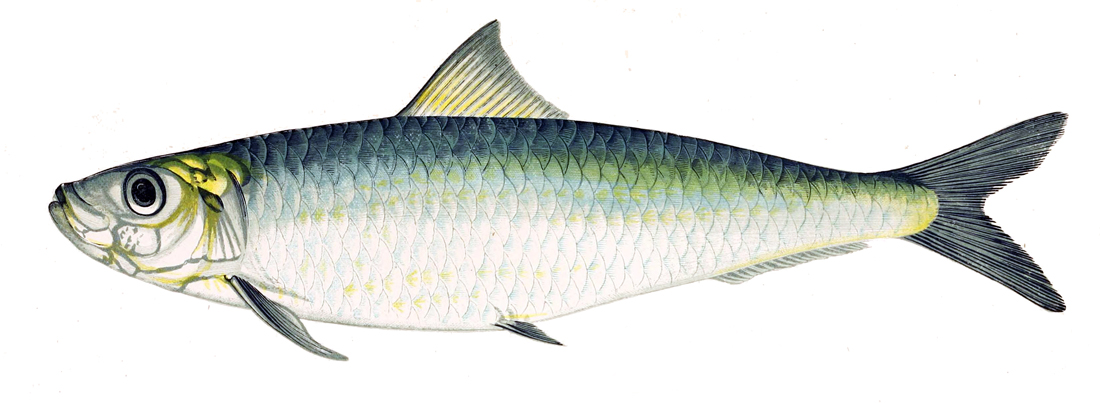
\includegraphics[scale=.3]{sardina_pilchardus_gervais}
  \end{figure}
\end{frame}
%--------------------------------------

%--------------------------------------
\begin{frame}{Sardinops Sagax Sagax}
  \begin{figure}
    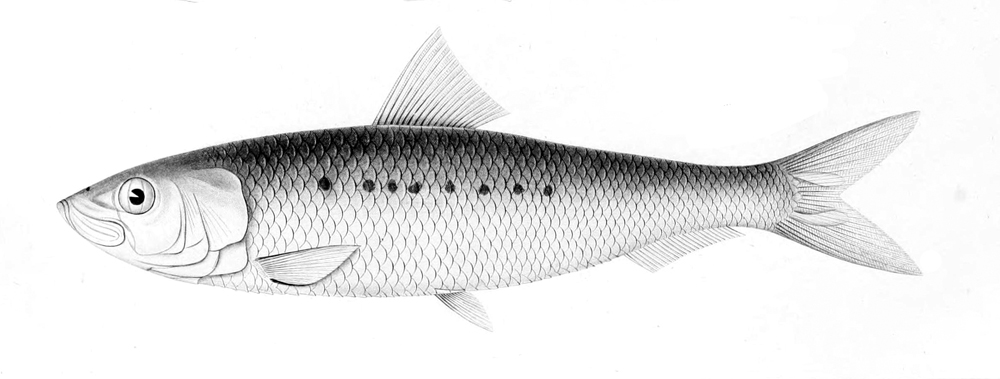
\includegraphics[scale=.3]{sardinops_sagax}
  \end{figure}
\end{frame}
%--------------------------------------

%--------------------------------------
\begin{frame}
 Fish determination according to the EU:\\ \medskip
 \textit{Sardina Pilchardus Gervais} $\rightarrow$ Sardine\\
 \textit{Sardinops Sagax Sagax} $\rightarrow$ Definitely not a sardine
\end{frame}
%--------------------------------------


%--------------------------------------
\begin{frame}
  Peru exported the \textit{sardinops sagax sagax} as sardines to the EU's common market.
  \begin{itemize}
    \item EU claimed however that this species of fish wasn't a sardine and therefore couldn't be traded under that name.
    \item Peru appealed to the WTO in 2001 claiming that this was a barrier to trade and a breach of the non-discrimination principle
  \end{itemize}
  \medskip
  The WTO panel concluded that indeed the EU regulation was inconsistent with WTO regulation and that the ban should be lifted
  \begin{itemize}
    \item In 2003 the EU lifted the import ban on Peruvian sardines, as well as other countries exporting the same fish
  \end{itemize}  
\end{frame}
%--------------------------------------

%--------------------------------------
\begin{frame}
 Next to the agreements set out by the WTO there are such things as preferential trade agreements
 \begin{itemize}
   \item Countries lower tariffs for each other but not third countries
 \end{itemize}
 \medskip
 This is a big no-no according to the WTO's MFN principle, save one exception
 \begin{enumerate}
   \item When the tariff is set to zero
 \end{enumerate}
\end{frame}
%--------------------------------------

%--------------------------------------
\begin{frame}  
  There are three types of preferential trade agreements
  \begin{enumerate}
    \item Free trade area, where there is free trade among members but a different policy towards non-members
    \item Customs union, where there is free trade among members and a common policy towards non-members
    \item Common market, which is a customs union combined with free movement of labour and capital
  \end{enumerate}
\end{frame}
%--------------------------------------

%--------------------------------------
\begin{frame}{Proliferation of regional trade agreements}
\framesubtitle{source: WTO}
  \begin{figure}
    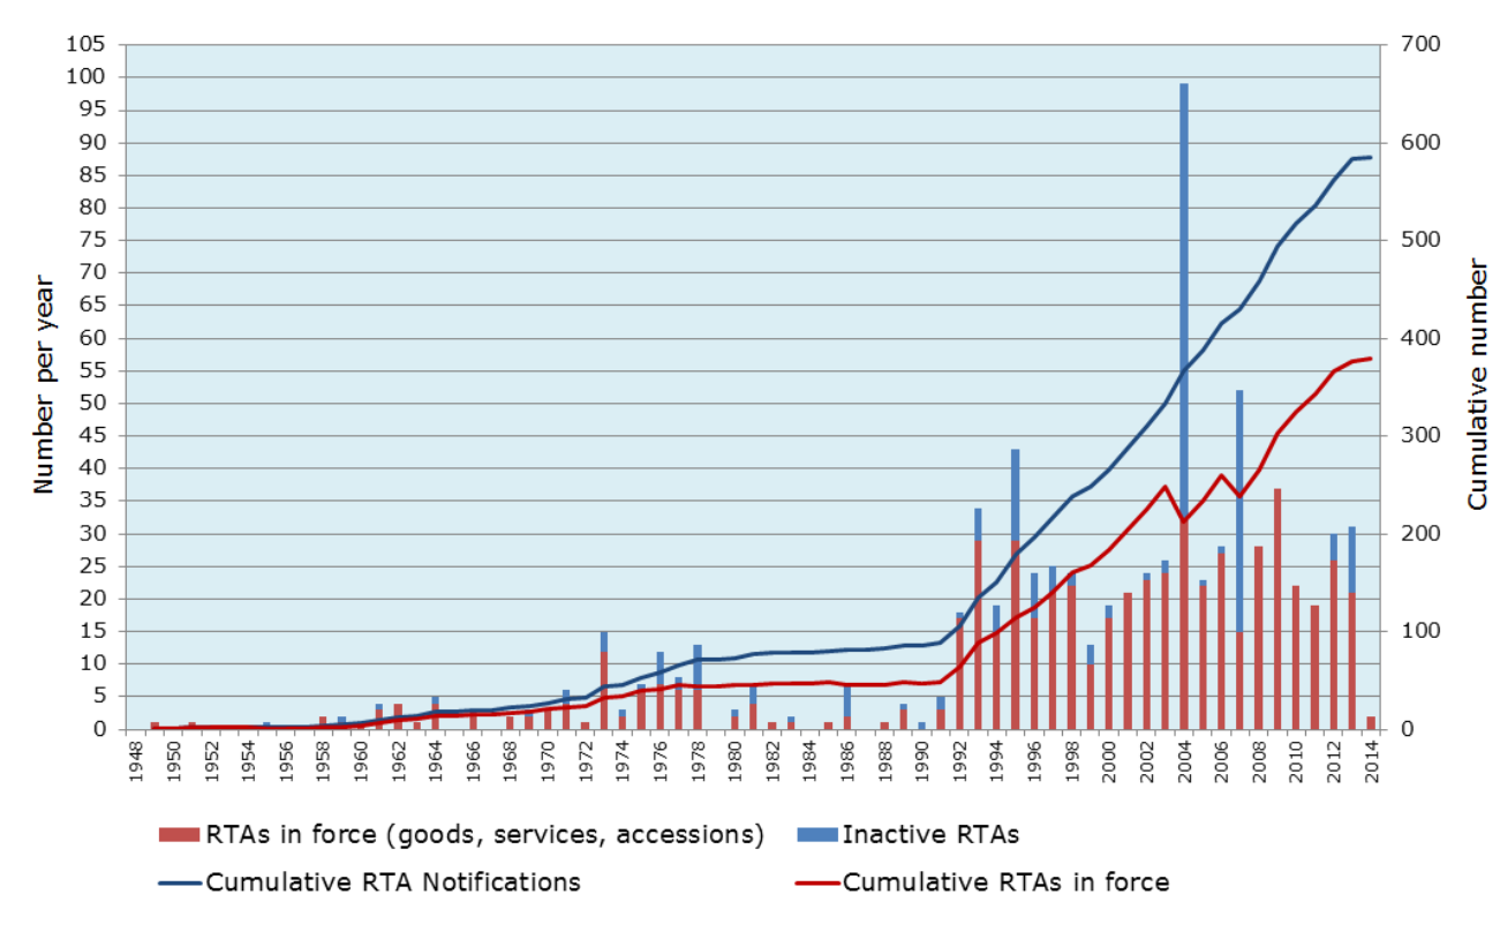
\includegraphics[scale=.8]{rta}
  \end{figure}
\end{frame}
%--------------------------------------

%--------------------------------------
\begin{frame}
  Regional trade agreements can have two divergent effects on trade
  \medskip
  \begin{enumerate}
    \item Trade creation, as lifting barriers allows cheaper imports from within region
    \begin{itemize}
      \item If prices are lower in partner countries compared to rest of the world      
    \end{itemize}
    \item Trade diversion, as lifting barriers discourages trade with rest of the world
    \begin{itemize}
      \item When prices are actually lower in the rest of the world
    \end{itemize}
  \end{enumerate}
\end{frame}
%--------------------------------------

%--------------------------------------
\begin{frame}
  \begin{figure}
    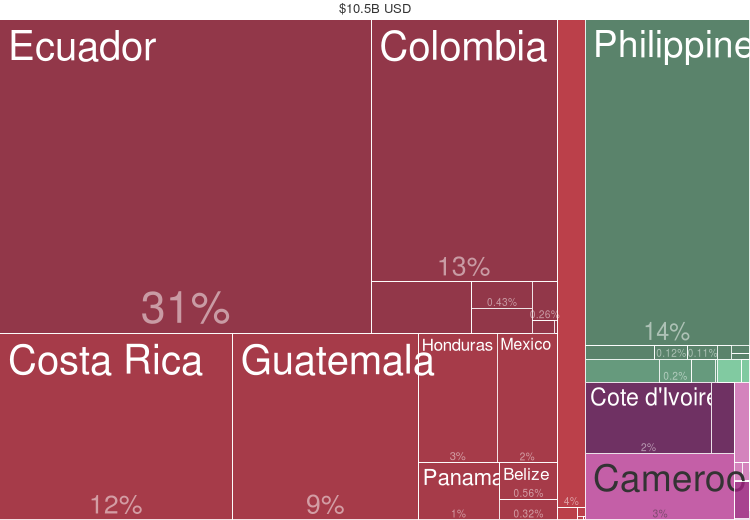
\includegraphics[scale=.4]{bananas}
  \end{figure}
\end{frame}
%--------------------------------------

%--------------------------------------
\begin{frame}
  In general most countries import bananas from Central America
  \begin{itemize}
    \item Ecuador, Costa Rica, Guatemala, etc.
  \end{itemize}
  \medskip
  The EU in contrast prefers to buy bananas from former colonies, the so called ACP countries (African, Caribbean, and Pacific)
  \begin{itemize}
    \item Belize, Cameroon, etc.
  \end{itemize}
  \medskip
  In order to protect the ACP imports, countries such as France and the UK imposed import quotas on Central American banana imports.  
\end{frame}
%--------------------------------------

%--------------------------------------
\begin{frame}
  In contrast, Germany did not import from these former ACP colonies initially, but was forced by EU rules to import the ACP bananas instead of the cheaper bananas from Central America; this upset some countries.
  \begin{itemize}
    \item Producing countries such as Equador and Guatemala
    \item and the USA because of corporate interest: Chiquita, Dole 
  \end{itemize}
  \medskip
  The USA was actually the country to file a complaint with the WTO which lead to what is now called the 20 year Banana War. 
\end{frame}
%--------------------------------------

%--------------------------------------
\begin{frame}
  In 1997 the WTO ruled that EU policy violated international trade rules, and in 2001 the EU and US agreed on phasing out banana quotas
  \begin{itemize}
    \item In 2005 the EU eliminated all import quotas but also tripled the tariffs
    \item The US retaliated by imposing 100\% import duties on a range of European products
  \end{itemize}
  \medskip
  In 2007 the WTO rules that the EU move was illegal and in 2009 the EU reduced the tariff from \texteuro 176 per tonne to \texteuro 114 per tonne
  \begin{itemize}
    \item In 2012 the EU and 10 Latin American countries signed an agreement to gradually reduce tariffs
  \end{itemize}
\end{frame}
%--------------------------------------

%--------------------------------------
\begin{frame}
  \begin{figure}
    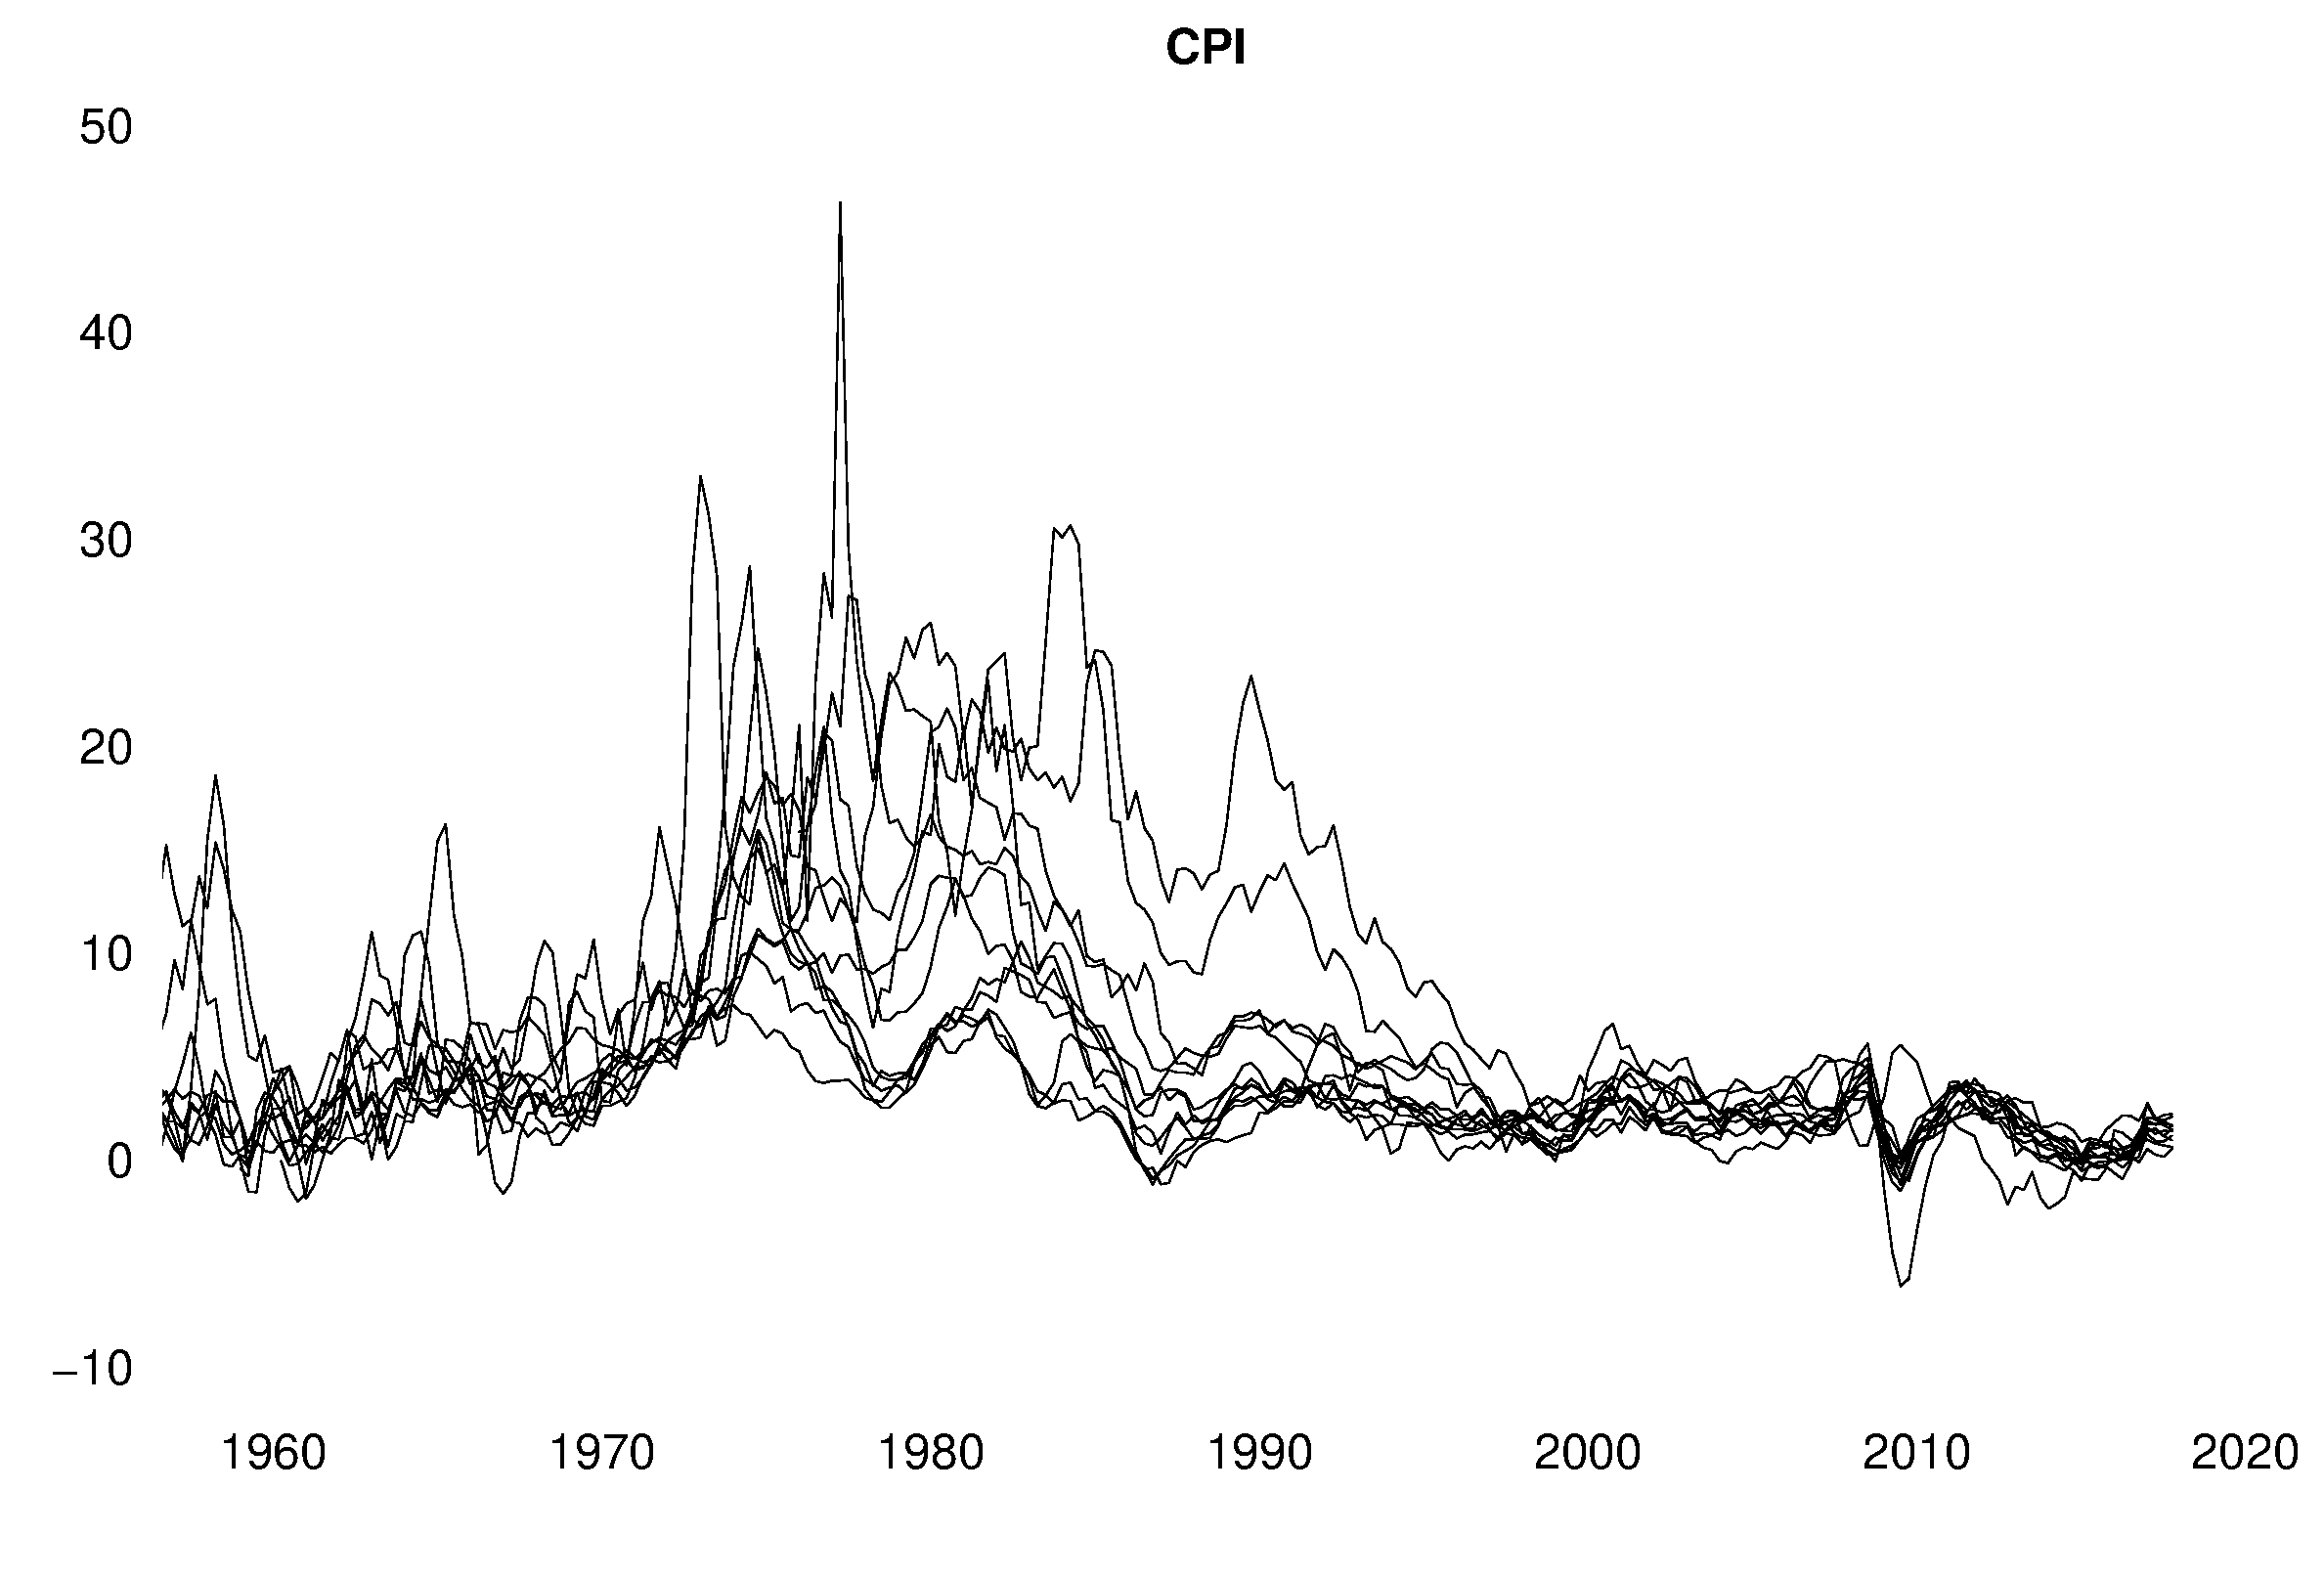
\includegraphics[scale=.3]{cpi.eps}
  \end{figure}
\end{frame}
%--------------------------------------

%--------------------------------------
\begin{frame}
  EU imposed economic sanctions on Russia in July 2014 in response to its destabilising actions in Eastern Ukraine.
  \begin{itemize}
    \item This followed the March annexation of the Crimea
  \end{itemize}
  \medskip
  The EU's economic sanctions focus predominantly on
  \begin{enumerate}
    \item Financial transactions
    \item Import/export of arms and military technology
    \item Exports of energy-related equipment and technology
  \end{enumerate}
  \medskip
  In response Russia banned fruit and vegetable imports from the EU
  \begin{itemize}
    \item As well as all food imports from the USA
  \end{itemize}
\end{frame}
%--------------------------------------

%--------------------------------------
\begin{frame}
  Trade sanctions and bans often take the form of action taken by one state, or by a group of states, to influence another state to change its behaviour.
  These actions generally involve restrictions on foreign trade or asset freezes and seizures. 
  \begin{itemize}
    \item US sanctions against Cuba or Iran
    \item UN sanctions against South Africa
    \item EU arms embargo on China
  \end{itemize}
  \medskip
  Sanctions can be preferred over straight military intervention as it is low cost and causes fewer deaths, but there are some disadvantages
  \begin{itemize}
    \item Probability of success might be low
    \item There are unintended consequences and indiscriminate effects which hurt innocent elements of society
  \end{itemize}
\end{frame}
%--------------------------------------

%--------------------------------------
\begin{frame}
  International trade can be used as a foreign policy tool given that trade is important for many countries
  \begin{itemize}
    \item Contributes substantially to GDP
    \item Countries can be dependent on trade for food and energy
  \end{itemize}
  \medskip
  It can be used both as a carrot and a stick.
  \begin{enumerate}
    \item Coercive policy tool to change certain behaviour of a state
    \item Influence domestic policy making, by intensifying trade relations    
  \end{enumerate}
\end{frame}
%--------------------------------------

%--------------------------------------
\begin{frame}
 For instance China uses trade as an instrument to influence foreign policy of foreign countries on issues that are important to China
 \begin{itemize}
   \item Recognition of Taiwan
   \item Human rights
 \end{itemize}
 \medskip
 For Latin American and African countries larger trade flows with China correspond with convergence on key foreign policy issues in UN voting.\footnote{"The Foreign Policy Consequences of Trade: China’s Commercial Relations with Africa and Latin America, 1992–2006", Flores-Macia \& Kreps, 2013, The Journal of Politics.}  
\end{frame}
%--------------------------------------

%--------------------------------------
\begin{frame}
  \begin{figure}
    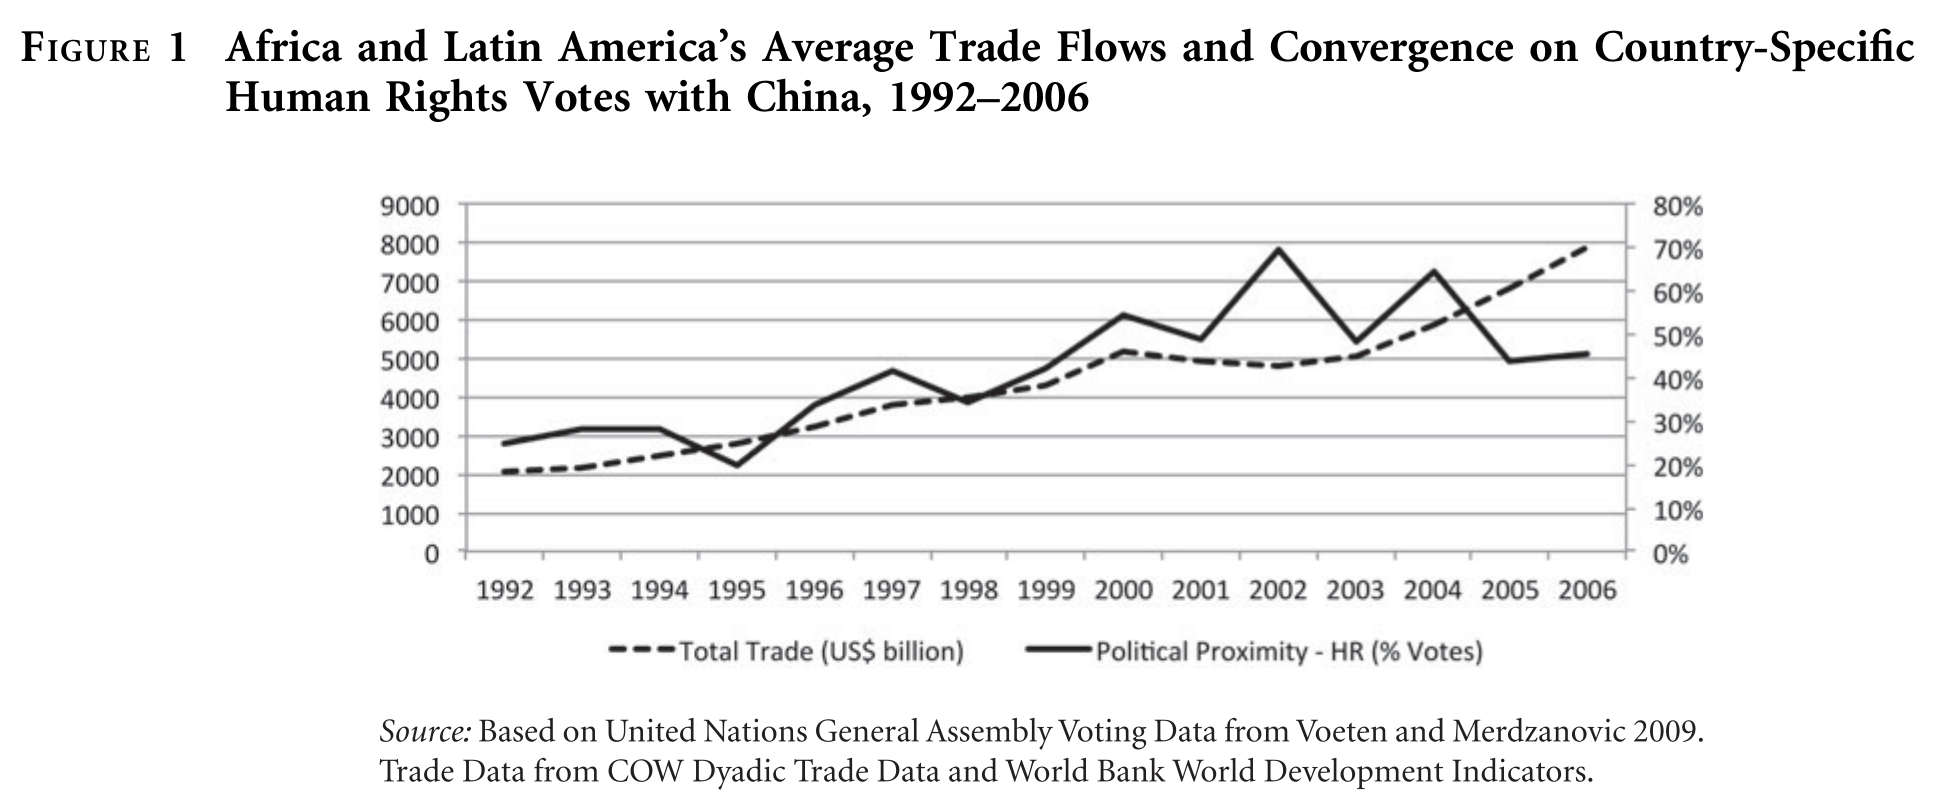
\includegraphics[scale=.7]{un_assembly1.png}
  \end{figure}  
\end{frame}
%--------------------------------------

%--------------------------------------
\begin{frame}
  \begin{figure}
    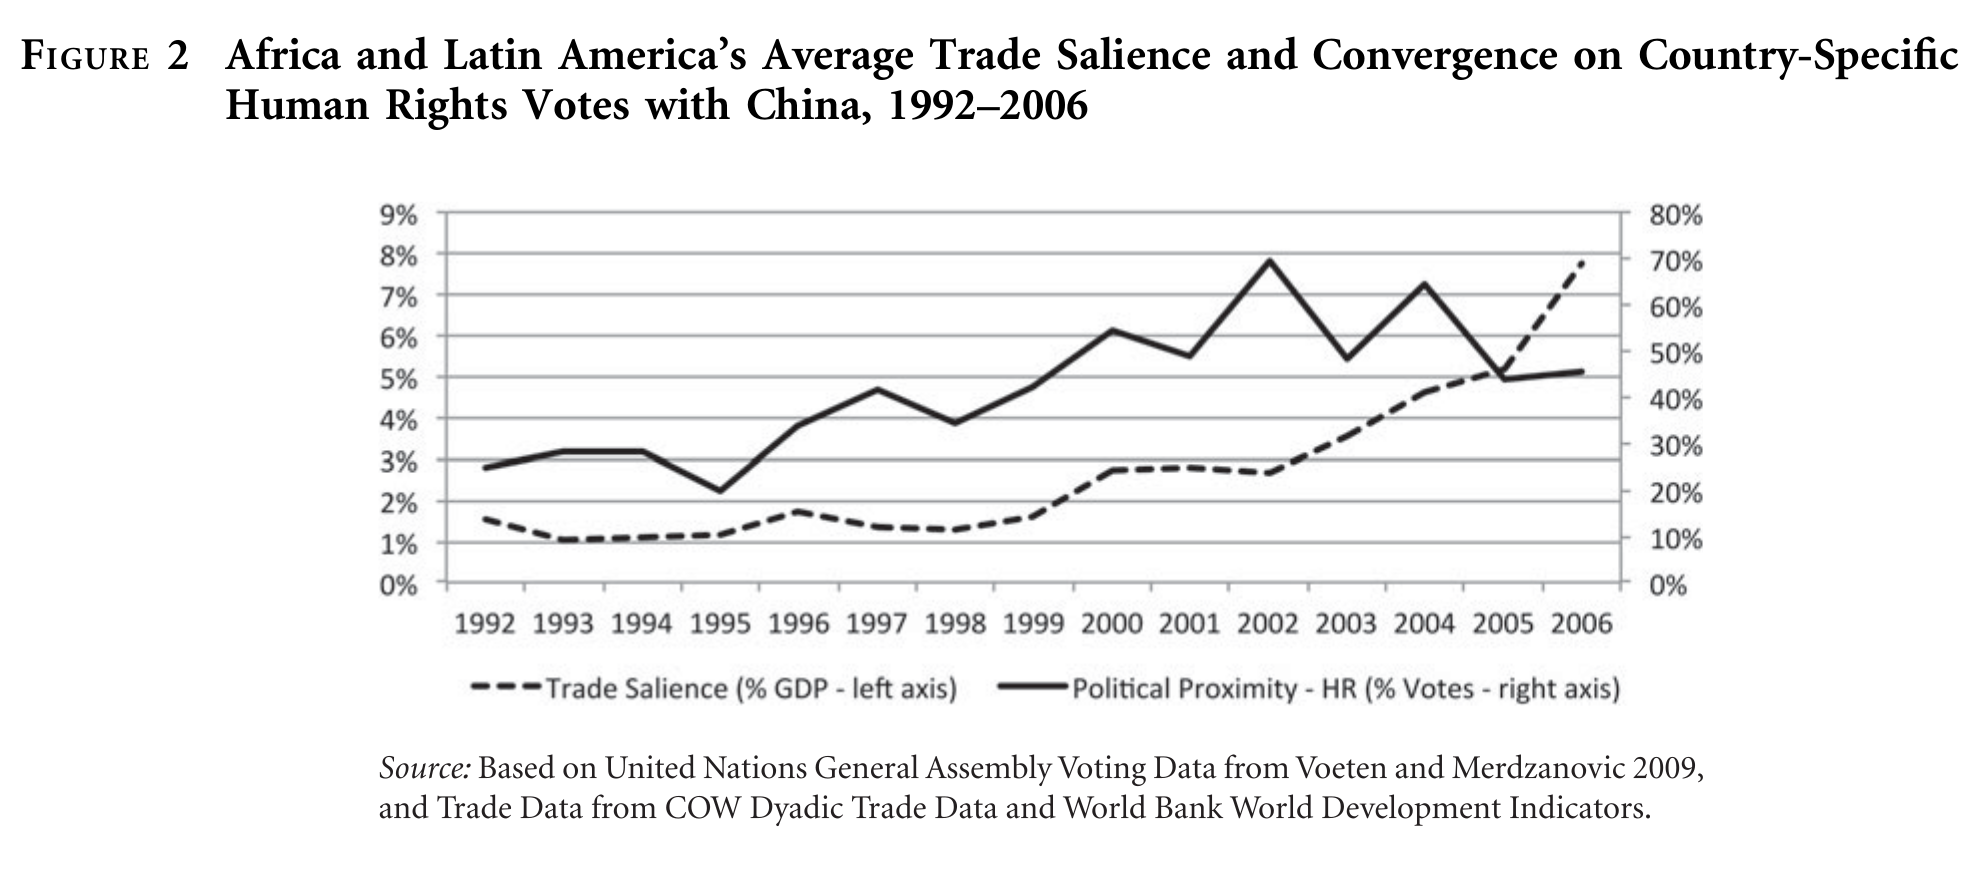
\includegraphics[scale=.7]{un_assembly2.png}
  \end{figure}  
\end{frame}
%--------------------------------------


%--------------------------------------
\begin{frame}
  The USA has used both overt and covers interventions to create larger foreign markets for American products.
  These interventions installed and supported political leaders that were supportive of the USA\footnote{"Commercial imperialism? Political influence and trade during the cold war", Berger \textit{et al.}, 2013, American Economic Review.}
  \begin{itemize}
    \item Intervention was followed by an increase in US imports, but not exports    
  \end{itemize}
  Moreover, the surge in imports is concentrated in sectors in which the USA had a comparative disadvantage
\end{frame}
%--------------------------------------

%--------------------------------------
\begin{frame}
  There is a conventional wisdom that trade has a pacifying effect and promotes peace
  \begin{itemize}
    \item EU result of preventing another war between France and Germany    
    \item MERCOSUR was created to curtail military power in Brazil and Argentina
  \end{itemize}
  \medskip
  Since the end WW2 there has been an increase in trade openness and decrease in interstate conflict. 
  International trade entails that countries can obtain resources without having to control territories.
  So question is whether more trade leads to fewer conflicts?
\end{frame}
%--------------------------------------

%--------------------------------------
\begin{frame}
  \begin{figure}
    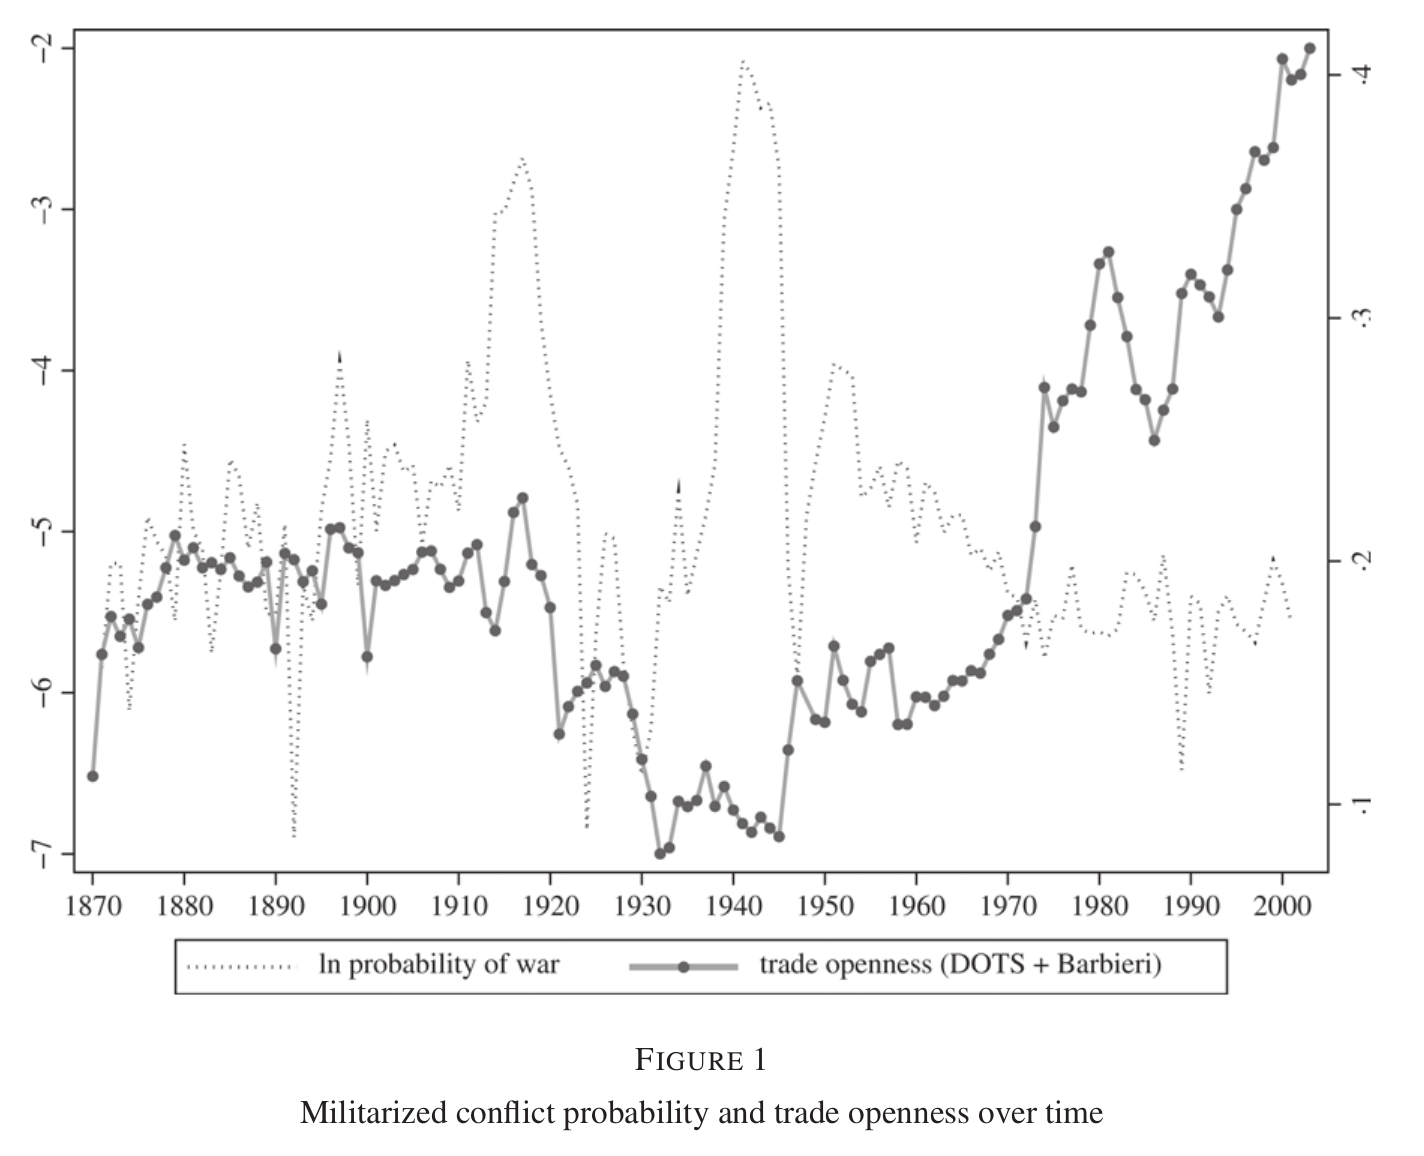
\includegraphics[scale=.7]{trade_war.png}
  \end{figure}
\end{frame}
%--------------------------------------

%--------------------------------------
\begin{frame}
  Conflict between countries is costly as it harms the economy, so bilateral trade certainly has the potential to reduce conflict probability
  \begin{itemize}
    \item Makes conflict costly as it creates dependence between countries    
  \end{itemize}
  \medskip
  Research suggests that for proximate countries bilateral trade reduces conflict risk by about 20\%.
  However, the trade-conflict nexus is asymmetric as multilateral trade increases the probability of interstate war
  \begin{itemize}
    \item Multilateral trade reduces bilateral dependence
    \item This reduces the cost of conflict and thus increases the probability
  \end{itemize}
\end{frame}
%--------------------------------------

%--------------------------------------
\begin{frame}
  There is some evidence that RTAs promote peaceful regions by increasing the opportunity cost of conflict and interestingly country pairs with a violence history are more likely to sign an RTA
  \begin{itemize}
    \item Larger pay-offs from signing a RTA
  \end{itemize}
  \medskip
  There are two types of peace promoting security gains from a RTA
  \begin{enumerate}
    \item Offering a political forum which facilitates settlement of future disputes
    \item Increase in opportunity costs of future potentially trade-disrupting wars
  \end{enumerate}
  \medskip
  Nonetheless, there does seem to be a larger conflict risk between member and non-member states
  \begin{itemize}
    \item A RTA also harms the multilateral trade system as it creates trade distortions for excluded members
  \end{itemize}
\end{frame}
%--------------------------------------


%------------------------------------------------------------------------------
\end{document}
